\section{Аналитический раздел}

\subsection{Постановка задачи}

В соответствии с заданием на курсовую работу необходимо разработать загружаемый модуль ядра, позволяющий осуществлять мониторинг выделения памяти в адресном пространстве ядра, предоставляющий информацию о запросах выделения физической памяти и выделения памяти в SLAB-кэше.
Для решения поставленной задачи необходимо решить следующие задачи:
\begin{enumerate}
    \item провести обзор способов выделения памяти в ядре Linux;
    \item провести обзор способов мониторинга выделения памяти;
    \item провести сравнительный анализ подходов к решению поставленной задачи;
    \item разработать алгоритмы и привести структуры данных для решения поставленной задачи;
    \item реализовать загружаемый модуль ядра, решающий поставленную задачу;
    \item протестировать разработанное программное обеспечение.
\end{enumerate}

\subsection{Выделение памяти в ядре Linux}

%Листинги функций и структур ядра Linux в данной работе будут приведены для версии ядра 6.6.

\subsubsection{NUMA}

Одним из наиболее распространенных понятий в управлении памятью является NUMA (англ. Non-Uniform Memory Access, неравномерный доступ к памяти или Non-Uniform Memory Architecture, архитектура с неравномерной памятью) --- архитектура организации компьютерной памяти, используемая в мультипроцессорных системах.
Процессор имеет быстрый доступ к локальной памяти через свой контроллер, а также более медленный канал до памяти, подключенной к контроллерам (слотам) других процессоров, реализуемый через шину обмена данными.~\cite{mem}
%Каждый процессор имеет собственный кэш.
%Межпроцессорное взаимодействие является частью архитектуры чипсетов, поэтому у каждого вендора своя реализация шины обмена данными.~\cite{mem}

На рисунке ниже приведена топология NUMA.

\begin{figure}[H]
	\centering
	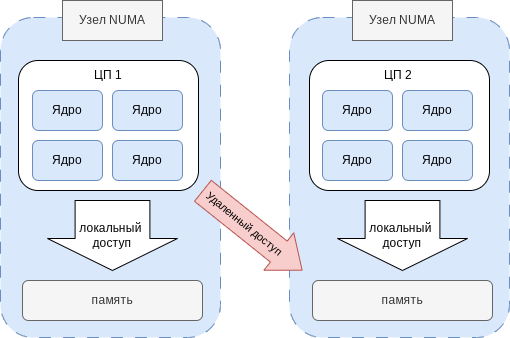
\includegraphics[width=0.9\textwidth]{img/numa.png}
	\caption{Топология NUMA}
	\label{fig:numa}
\end{figure}

То есть, каждый узел NUMA содержит:
\begin{enumerate}
    \item CPU (или несколько ядер);
    \item Локальную память (RAM);
    \item Контроллер памяти.
\end{enumerate}

Если процесс выполняется на CPU и запрашивает память из другого NUMA-узла, доступ к ней будет медленнее, чем если бы эта память была выделена из локального узла.
Поэтому ядро Linux старается выделять память из локального узла.

%Каждый процессор архитектуры NUMA может получить доступ к своей собственной памяти и памяти других процессоров.
%Доступ к своей собственной памяти намного быстрее, чем доступ к другой памяти, с разницей в скорости в 10-100 раз.
%Поэтому целью настройки NUMA является предоставление процессору максимально возможного доступа к собственной памяти для повышения скорости доступа.~\cite{numatop}

\subsubsection{NUMA, узлы памяти и зоны в Linux}

В многопроцессорных (англ. multi-core) и многосокетных (англ. multi-socket) системах память может быть организована в банки, доступ к которым имеет разную стоимость в зависимости от их <<удалённости>> от процессора.
Например, может существовать банк памяти, закреплённый за каждым процессором, или банк памяти, предназначенный для DMA, расположенный рядом с периферийными устройствами.

Каждый такой банк памяти называется узлом (англ. node).
В Linux банк представлен структурой {struct pglist\_data}, даже если архитектура является UMA (англ. Uniform Memory Access, равномерный доступ к памяти).
Эта структура всегда используется через {typedef pg\_data\_t}.
Чтобы получить структуру {pg\_data\_t} для конкретного узла, используется макрос {NODE\_DATA(nid)}, где {nid} — это идентификатор (ID) узла.

Ниже приведен листинг структуры pg\_data\_t из ядра Linux версии 6.6.

\begin{lstlisting}[caption={struct pglist\_data}]
typedef struct pglist_data {
	struct zone node_zones[MAX_NR_ZONES];
	struct zonelist node_zonelists[MAX_ZONELISTS];

    /* number of populated zones in this node */
	int nr_zones;
    ...
	unsigned long node_start_pfn;

    /* total number of physical pages */
	unsigned long node_present_pages;

    /* total size of physical page range, including holes */
	unsigned long node_spanned_pages;
	int node_id;
    ...
	/*
	 * This is a per-node reserve of pages that are not available
	 * to userspace allocations.
	 */
	unsigned long		totalreserve_pages;

#ifdef CONFIG_NUMA
	/*
	 * node reclaim becomes active if more unmapped pages exist.
	 */
	unsigned long		min_unmapped_pages;
	unsigned long		min_slab_pages;
#endif /* CONFIG_NUMA */
    ...
} pg_data_t;
\end{lstlisting}

В архитектурах NUMA структуры узлов создаются специфичным для архитектуры кодом на ранних этапах загрузки системы (boot).
Обычно эти структуры выделяются локально на банков памяти, который они представляют.
В архитектурах UMA используется только одна статическая структура {pg\_data\_t}, называемая {contig\_page\_data}.

Всё физическое адресное пространство разделено на один или несколько блоков, называемых зонами (англ. zones), которые представляют диапазоны памяти.
Эти диапазоны обычно определяются аппаратными ограничениями на доступ к физической памяти.
Внутри каждого узла определённая зона памяти описывается с помощью структуры {struct zone}.~\cite{mem}

\subsubsection{Зоны в Linux}

Каждый NUMA-узел разделяется на зоны (ZONE\_*), чтобы учитывать аппаратные ограничения:

\begin{enumerate}
    \item ZONE\_DMA и ZONE\_DMA32 исторически представляют области памяти, подходящие для DMA-операций (Direct Memory Access) периферийных устройств, которые не могут обращаться ко всей адресуемой памяти;
    \item ZONE\_NORMAL предназначена для обычной памяти, к которой ядро всегда имеет доступ;
    \item ZONE\_HIGHMEM --- это часть физической памяти, которая не отображается постоянно в таблицы страниц ядра. Доступ к памяти в этой зоне возможен только с использованием временных отображений (temporary mappings). Эта зона применяется только в некоторых 32-битных архитектурах;
    \item ZONE\_MOVABLE --- это зона обычной памяти, но её содержимое можно перемещать (для оптимизации фрагментации);
    \item ZONE\_DEVICE предназначена для памяти, находящейся на устройствах (например, постоянная память PMEM или память GPU). Эта память имеет другие характеристики, отличающиеся от обычной оперативной памяти (RAM). ZONE\_DEVICE используется, чтобы предоставить драйверам устройств структуры {struct page} и механизмы управления памятью для работы с физическими адресами, определенными устройством.~\cite{mem}
\end{enumerate}

\subsubsection{Структура struct page и массив mem\_map}

В ядре Linux каждая физическая страница памяти представляется структурой {struct page}, содержащей метаданные, необходимые для её управления.
Все структуры {struct page} организованы в массив {mem\_map}, который создаётся при инициализации системы и позволяет ядру отслеживать и управлять всей физической памятью.

Массив mem\_map обеспечивает быстрый доступ к структуре {struct page} по номеру страницы (PFN, Page Frame Number).

Далее представлен листинг структуры {struct page}.

\begin{lstlisting}[caption={struct page}]
struct page {
    /* Atomic flags, some possibly updated asynchronously */
	unsigned long flags;
	/*
	 * Five words (20/40 bytes) are available in this union.
	 * WARNING: bit 0 of the first word is used for PageTail(). That
	 * means the other users of this union MUST NOT use the bit to
	 * avoid collision and false-positive PageTail().
	 */
	union {
		struct {	/* Page cache and anonymous pages */
			/**
			 * @lru: Pageout list, eg. active_list protected by
			 * lruvec->lru_lock.  Sometimes used as a generic list
			 * by the page owner.
			 */
			union {
				struct list_head lru;
				/* Or, for the Unevictable "LRU list" slot */
				struct {
					/* Always even, to negate PageTail */
					void *__filler;
					/* Count page's or folio's mlocks */
					unsigned int mlock_count;
				};
				/* Or, free page */
				struct list_head buddy_list;
				struct list_head pcp_list;
			};
			/* See page-flags.h for PAGE_MAPPING_FLAGS */
			struct address_space *mapping;
			union {
				pgoff_t index;		/* Our offset within mapping. */
				unsigned long share;	/* share count for fsdax */
			};
			/**
			 * @private: Mapping-private opaque data.
			 * Usually used for buffer_heads if PagePrivate.
			 * Used for swp_entry_t if PageSwapCache.
			 * Indicates order in the buddy system if PageBuddy.
			 */
			unsigned long private;
		};
        ...
		struct {	/* ZONE_DEVICE pages */
			/** @pgmap: Points to the hosting device page map. */
			struct dev_pagemap *pgmap;
			void *zone_device_data;
			/*
			 * ZONE_DEVICE private pages are counted as being
			 * mapped so the next 3 words hold the mapping, index,
			 * and private fields from the source anonymous or
			 * page cache page while the page is migrated to device
			 * private memory.
			 * ZONE_DEVICE MEMORY_DEVICE_FS_DAX pages also
			 * use the mapping, index, and private fields when
			 * pmem backed DAX files are mapped.
			 */
		};

		/** @rcu_head: You can use this to free a page by RCU. */
		struct rcu_head rcu_head;
	};

	union {		/* This union is 4 bytes in size. */
		/*
		 * If the page can be mapped to userspace, encodes the number
		 * of times this page is referenced by a page table.
		 */
		atomic_t _mapcount;
		/*
		 * If the page is neither PageSlab nor mappable to userspace,
		 * the value stored here may help determine what this page
		 * is used for.  See page-flags.h for a list of page types
		 * which are currently stored here.
		 */
		unsigned int page_type;
	};
    ...
	/*
	 * On machines where all RAM is mapped into kernel address space,
	 * we can simply calculate the virtual address. On machines with
	 * highmem some memory is mapped into kernel virtual memory
	 * dynamically, so we need a place to store that address.
	 * Note that this field could be 16 bits on x86 ... ;)
	 *
	 * Architectures with slow multiplication can define
	 * WANT_PAGE_VIRTUAL in asm/page.h
	 */
#if defined(WANT_PAGE_VIRTUAL)
	void *virtual;			/* Kernel virtual address (NULL if
					   not kmapped, ie. highmem) */
#endif /* WANT_PAGE_VIRTUAL */
    ...
};
\end{lstlisting}

На рисунке ниже представлено отношение между узлами памяти, зонами и страницами.

\begin{figure}[H]
	\centering
	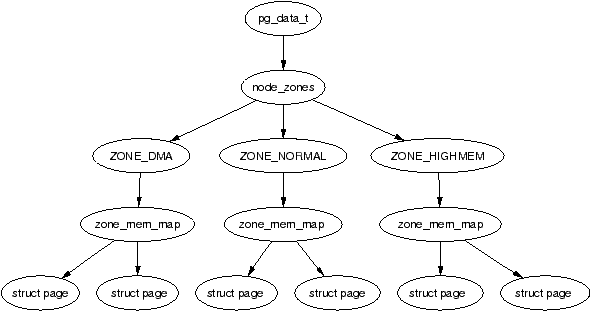
\includegraphics[width=0.9\textwidth]{img/zones.png}
	\caption{Отношение между узлами памяти, зонами и страницами~\cite{pmem}}
	\label{fig:pmem}
\end{figure}

%\subsection{SLAB-кэш}
\subsubsection{SLAB-кэш}

Выделение памяти через buddy allocator (используемый для {alloc\_pages()}) неэффективно для мелких объектов, поскольку:
\begin{itemize}
    \item Использование целых страниц для маленьких структур ведет к фрагментации;
    \item Buddy-аллокатор медленный при работе с большим количеством небольших объектов.
\end{itemize}

SLAB-аллокатор решает эту проблему, создавая пулы (SLAB-кэши) для повторного использования объектов одного типа.

SLAB-аллокатор --- это механизм управления динамической памятью в ядре Linux, предназначенный для эффективного выделения и повторного использования объектов фиксированного размера (например, task\_struct, inode, dentry).
Он является частью системы управления памятью и предназначен для работы с небольшими объектами, которые часто выделяются и освобождаются.

Работает аллокатор следующим образом:
\begin{enumerate}
    %\item Каждый тип объекта (например, struct task\_struct) получает свой SLAB-кэш (kmem\_cache);
    %\item При запросе памяти ядро выделяет сразу несколько объектов (batch allocation);
    \item Ядро создает кэш (kmem\_cache\_create()) для типа объектов (например, task\_struct);
    \item SLAB-аллокатор выделяет группу объектов сразу и хранит их в struct slab;
    \item При kmem\_cache\_alloc() ядро берет объект из кэша, а не выделяет память заново;
    \item Когда объект освобождается (kmem\_cache\_free()) --- возвращается в кэш, а не в buddy allocator;
    \item Если в кэше не осталось свободных объектов, SLAB-аллокатор запрашивает новые страницы через alloc\_pages().
\end{enumerate}

\subsubsection{Структуры {struct kmem\_cache} и {struct slab}}

Ниже приведены структуры ядра {struct kmem\_cache} и {struct slab}, используемые при работе со SLAB-аллокатором.

\begin{lstlisting}[caption={struct kmem\_cache}]
struct kmem_cache {
	struct array_cache __percpu *cpu_cache;
    ...
	unsigned int size;
    ...
	slab_flags_t flags;		/* constant flags */
	unsigned int num;		/* # of objs per slab */
    ...
	const char *name;
	struct list_head list;
	int refcount;
	int object_size;
	int align;
    ...
	struct kmem_cache_node *node[MAX_NUMNODES];
};
\end{lstlisting}

\begin{lstlisting}[caption={struct slab}]
struct slab {
	unsigned long __page_flags;
#if defined(CONFIG_SLAB)
	struct kmem_cache *slab_cache;
	union {
		struct {
			struct list_head slab_list;
			void *freelist;	/* array of free object indexes */
			void *s_mem;	/* first object */
		};
		struct rcu_head rcu_head;
	};
	unsigned int active;
    ...
#elif defined(CONFIG_SLUB)
	struct kmem_cache *slab_cache;
	union {
		struct {
			union {
				struct list_head slab_list;
                ...
			};
			/* Double-word boundary */
			union {
				struct {
					void *freelist;		/* first free object */
					union {
						unsigned long counters;
						struct {
							unsigned inuse:16;
							unsigned objects:15;
							unsigned frozen:1;
						};
					};
				};
                ...
			};
		};
		struct rcu_head rcu_head;
	};
    ...
#endif
};
\end{lstlisting}


\subsection{Функции и системные вызовы}

Для работы с памятью в ядре Linux предусмотрены функции
\begin{itemize}
    \item alloc\_pages,
    \item kmem\_cache\_create,
    \item kmem\_cache\_alloc,
    \item kmem\_cache\_free,
    \item kmem\_cache\_destroy,
    \item kmalloc, kfree
\end{itemize}
и другие.

\subsubsection{alloc\_pages}

Функция alloc\_pages() вызывает основную функцию выделения страниц --- \_\_alloc\_pages(), которая выполняет несколько шагов:
\begin{enumerate}
    \item Выбор зоны памяти;
    \item Поиск подходящего блока в buddy allocator;
    \item Выделение памяти.
\end{enumerate}

\subsubsection*{Выбор зоны памяти}

Выбор зоны памяти происходит следующим образом --- \_\_alloc\_pages() определяет, из какой зоны (ZONE\_*) выделять память:
\begin{itemize}
    \item ZONE\_DMA;
    \item ZONE\_NORMAL;
    \item ZONE\_HIGHMEM;
    \item ZONE\_MOVABLE;
    \item ZONE\_DEVICE;
\end{itemize}

После чего функция get\_page\_from\_freelist() ищет свободные страницы в нужной зоне:
\begin{lstlisting}
struct page *page = get_page_from_freelist(gfp_mask, order, alloc_flags, alloc_context);
\end{lstlisting}

\subsubsection*{Поиск подходящего блока в buddy allocator}

Buddy allocator хранит свободные страницы в списках (free\_area).

\begin{enumerate}
    \item Если есть подходящий свободный блок, то этот блок разбивается и выделяется.
    \item Если нет свободного блока нужного размера, система ищет больше страниц.
    \item Если памяти недостаточно, включается свопинг (swap) или OOM-Killer.
\end{enumerate}

Buddy allocator выделяет память вызовом remove\_from\_free\_list():
\begin{lstlisting}
page = remove_from_free_list(zone, order);
\end{lstlisting}

Причем если
\begin{itemize}
    \item order = 0 --- выделяется 1 страница;
    \item order = 1 --- выделяется 2 страницы ($2^1$);
    \item order = 2 --- выделяется 4 страницы ($2^2$)
\end{itemize}
и так далее.

\subsubsection*{Выделение памяти}

Если найдена свободная страница, ядро
\begin{itemize}
\item Помечает её как занятую (PageReserved);
\item Обновляет структуру struct page, устанавливая флаги и счётчик ссылок;
\item Возвращает struct page *;
\end{itemize}

После чего функция prep\_new\_page() инициализирует страницу:
\begin{lstlisting}
if (page) prep_new_page(page, order, gfp_mask);
\end{lstlisting}

\subsubsection{kmem\_cache\_*}

Далее будут рассмотрены функции kmem\_cache\_alloc, kmem\_cache\_free, kmem\_cache\_create, kmem\_cache\_destroy.

\subsubsection*{kmem\_cache\_create}

Данная функия предназначена для создания SLAB-кэша.

\begin{lstlisting}
struct kmem_cache *kmem_cache_create(const char *name, size_t size, size_t align, slab_flags_t flags, void (*ctor)(void *));
\end{lstlisting}

Аргументы:
\begin{enumerate}
    \item name --- Имя кэша (отображается в /proc/slabinfo);
    \item size --- Размер объекта в байтах;
    \item align	--- Выравнивание объекта (0 --- авто);
    \item flags	--- Флаги SLAB (SLAB\_HWCACHE\_ALIGN, SLAB\_PANIC);
    \item ctor --- Функция-конструктор (инициализация объекта, может быть NULL).
\end{enumerate}

Данная функция
\begin{itemize}
    \item Выделяет SLAB-кэш для объектов одного типа;
    \item Создаёт struct kmem\_cache, которая управляет списком объектов;
    \item Создаёт SLAB-пулы (struct slab).
    %\item Если используется SLAB, создаёт SLAB-пулы (struct slab);
    %\item Если SLUB, создаёт структуры на основе struct page.
\end{itemize}

Пример создания кэша для task\_struct:

\begin{lstlisting}
struct kmem_cache *task_struct_cache;
task_struct_cache = kmem_cache_create("task_struct_cache", sizeof(struct task_struct), 0, SLAB_HWCACHE_ALIGN, NULL);
\end{lstlisting}

\subsubsection*{kmem\_cache\_alloc}

Данная функция предназначена для выделения объекта из SLAB-кэша.
\begin{lstlisting}
void *kmem_cache_alloc(struct kmem_cache *cachep, gfp_t flags);
\end{lstlisting}

Аргументы:
\begin{enumerate}
    \item cachep --- Указатель на кэш (struct kmem\_cache *);
    \item flags --- Флаги выделения памяти (GFP\_KERNEL, GFP\_ATOMIC).
\end{enumerate}

Данная функция
\begin{itemize}
    \item Ищет свободный объект в kmem\_cache;
    \item Если кэш пуст, вызывает alloc\_pages() для выделения новых страниц;
    \item Возвращает указатель на объект.
\end{itemize}

Пример выделения объекта кэша для task\_struct:

\begin{lstlisting}
struct task_struct *task = kmem_cache_alloc(task_struct_cache, GFP_KERNEL);
\end{lstlisting}

\subsubsection*{kmem\_cache\_free}

Данная функция предназначена для освобождения объекта.

\begin{lstlisting}
void kmem_cache_free(struct kmem_cache *cachep, void *objp);
\end{lstlisting}

Аргументы:
\begin{enumerate}
    \item cachep --- Указатель SLAB-кэш;
    \item objp --- Указатель на объект, который нужно освободить.
\end{enumerate}

Данная функция
\begin{itemize}
    \item Добавляет объект обратно в кэш;
    \item Если кэш заполнен, объект возвращается в buddy allocator;
    \item Если используется SLAB, объект остаётся в struct slab.
\end{itemize}

Пример освобождения task\_struct:

\begin{lstlisting}
kmem_cache_free(task_struct_cache, task);
\end{lstlisting}

\subsubsection*{kmem\_cache\_destroy}

Данная функция предназначена для удаления SLAB-кэша.

\begin{lstlisting}
void kmem_cache_destroy(struct kmem_cache *cachep);
\end{lstlisting}

Аргументы:
\begin{itemize}
    \item cachep --- Указатель на struct kmem\_cache;
\end{itemize}

Данная функция
\begin{itemize}
    \item Освобождает все объекты в кэше;
    \item Возвращает все занятые страницы в buddy allocator;
    \item Удаляет kmem\_cache из списка SLAB-кэшей.
\end{itemize}

Пример удаления кэша:

\begin{lstlisting}
kmem_cache_destroy(task_struct_cache);
\end{lstlisting}

\subsubsection{kmalloc}

Функция kmalloc() используется для выделения памяти в пространстве ядра и работает через SLAB-аллокатор или buddy allocator, в зависимости от размера запроса и конфигурации системы.

\begin{lstlisting}
void *kmalloc(size_t size, gfp_t flags);
\end{lstlisting}

Аргументы:
\begin{itemize}
    \item size --- Размер выделяемой памяти (в байтах);
    \item flags --- Флаги выделения памяти (GFP\_KERNEL, GFP\_ATOMIC и т. д.).
\end{itemize}

Функция kmalloc() может работать через разные механизмы, в зависимости от размера запроса.
Так для маленьких объектов (size $\leq$ PAGE\_SIZE) выделение происходит через SLAB, а для больших объектов (size > PAGE\_SIZE) выделение происходит через alloc\_pages().

Ниже представлены листинги функций kmalloc, \_\_kmalloc и kmalloc\_large.

\begin{lstlisting}[caption={kmalloc}]
void *kmalloc(size_t size, gfp_t flags)
{
    return __kmalloc(size, flags);
}
\end{lstlisting}

\begin{lstlisting}[caption={\_\_kmalloc}]
void *__kmalloc(size_t size, gfp_t flags)
{
    struct kmem_cache *cache;
    cache = kmalloc_slab(size, flags);
    if (unlikely(!cache))
        return kmalloc_large(size, flags);
    return kmem_cache_alloc(cache, flags);
}
\end{lstlisting}

\begin{lstlisting}[caption={kmalloc\_large}]
static void *kmalloc_large(size_t size, gfp_t flags)
{
    struct page *page;
    page = alloc_pages(flags, get_order(size));
    if (!page)
        return NULL;
    return page_address(page);
}
\end{lstlisting}

Функция kmalloc\_slab() находит нужный SLAB-кэш (kmalloc-32, kmalloc-64, kmalloc-128 и т.д.), после чего, если есть свободные объекты, они выделяются через kmem\_cache\_alloc().

\subsubsection*{Примеры использования kmalloc}

\begin{lstlisting}[caption={Выделение памяти в SLAB-кэше}]
void *ptr = kmalloc(64, GFP_KERNEL);
if (!ptr) printk(KERN_ERR "kmalloc\n");
\end{lstlisting}

\begin{lstlisting}[caption={Выделение памяти через alloc\_pages}]
void *ptr = kmalloc(8192, GFP_KERNEL);
\end{lstlisting}

\subsubsection{kfree}

Функция kfree() освобождает память.
Если память была выделена через SLAB, объект возвращается в SLAB-кэш.
Если память была выделена через alloc\_pages(), страницы освобождаются через \_\_free\_pages().

\begin{lstlisting}[caption={kfree}]
kfree(ptr);
\end{lstlisting}

\subsection{Анализ способов мониторинга памяти}

Мониторинг выделения и использования памяти в ядре Linux может осуществляться разными способами, включая перехват системных вызовов и хуки ядра, а также использование встроенных системных интерфейсов.

%\subsubsection*{Перехват системных вызовов и хуки ядра}

Существует множество способов перехвата системных вызовов.
%Далее будут рассмотрены самые распространенные --- kprobes, tracepoints, ftrace, perf и eBPF.
Далее будут рассмотрены самые распространенные --- kprobes, tracepoints и ftrace.

\subsubsection*{kprobes}

Механизм kprobes позволяет динамически устанавливать точки останова в любую функцию ядра и собирать отладочную информацию без нарушения работы системы.
С помощью него возможно перехватывать практически любой адрес в коде ядра, указывая обработчик, который будет вызван при срабатывании точки останова.~\cite{kprobe}

В настоящее время существует два типа проб (probes):
\begin{enumerate}
    \item kprobes --- стандартные точки перехвата, которые можно вставить практически в любую инструкцию ядра;
    \item kretprobes (return probes) --- перехватывают момент выхода из указанной функции (при её возврате).
\end{enumerate}

Обычно kprobes используется в виде загружаемого модуля ядра.
Функция инициализации модуля устанавливает (регистрирует) одну или несколько kprobe.
Функция выхода удаляет их.
Регистрация выполняется с помощью функции register\_kprobe(), в которой указывается адрес точки перехвата и обработчик, который должен выполниться при её срабатывании.~\cite{kprobe}

Ниже приведена структура struct kprobe.

\begin{lstlisting}[caption={struct kprobe}]
struct kprobe {
	struct hlist_node hlist;

	/* list of kprobes for multi-handler support */
	struct list_head list;

	/*count the number of times this probe was temporarily disarmed */
	unsigned long nmissed;

	/* location of the probe point */
	kprobe_opcode_t *addr;

	/* Allow user to indicate symbol name of the probe point */
	const char *symbol_name;

	/* Offset into the symbol */
	unsigned int offset;

	/* Called before addr is executed. */
	kprobe_pre_handler_t pre_handler;

	/* Called after addr is executed, unless... */
	kprobe_post_handler_t post_handler;

	/* Saved opcode (which has been replaced with breakpoint) */
	kprobe_opcode_t opcode;

	/* copy of the original instruction */
	struct arch_specific_insn ainsn;

	/* Indicates various status flags.
	 * Protected by kprobe_mutex after this kprobe is registered.
	 */
	u32 flags;
};
\end{lstlisting}

Пример загружаемого модуля ядра, использующего kprobes для перехвата kmalloc():
\begin{lstlisting}
#include <linux/kprobes.h>
#include <linux/module.h>
#include <linux/slab.h>

static int handler_pre(struct kprobe *p, struct pt_regs *regs) {
    size_t size = regs->di;
    printk(KERN_INFO "kmalloc called: size = %zu bytes\n", size);
    return 0;
}

static struct kprobe kp = {
    .symbol_name = "__kmalloc",
    .pre_handler = handler_pre,
};

static int __init kprobe_init(void) {
    int ret = register_kprobe(&kp);
    if (ret < 0) {
        pr_err("Failed to register kprobe: %d\n", ret);
        return ret;
    }
    pr_info("kprobe for kmalloc installed\n");
    return 0;
}

static void __exit kprobe_exit(void) {
    unregister_kprobe(&kp);
    pr_info("kprobe removed\n");
}

module_init(kprobe_init);
module_exit(kprobe_exit);
\end{lstlisting}

\subsubsection*{tracepoints}

Точка трассировки (tracepoint), размещённая в коде, предоставляет возможность вызвать функцию (пробу, probe), которую можно назначить во время выполнения.
Если tracepoint <<включен>> (к нему подключена probe), то при его срабатывании вызывается соответствующая функция.
Если tracepoint <<выключен>> (к нему не подключено обработчиков), то точка трассировки не влияет на выполнение кода, за исключением небольшой временной задержки и небольших затрат памяти.
Функция-проба вызывается каждый раз при выполнении tracepoint.
Выполняется в том же контексте, что и вызывающая функция.
После завершения работы обработчика выполнение возвращается в исходное место, продолжая выполнение основной программы.

Точки трассировки используются для трассировки и анализа производительности.
Их можно вставлять в критически важные участки кода, чтобы отслеживать работу системы.~\cite{tracepoints}

% TODO: meybi ed samfing from hier: https://www.kernel.org/doc/html/latest/trace/tracepoints.html

\subsubsection*{ftrace}

Ftrace --- это фреймворк, состоящий из нескольких различных утилит трассировки.
Одно из самых распространенных применений ftrace --- трассировка событий.
По всему ядру расположены сотни статических точек событий, которые можно включить через файловую систему tracefs, чтобы посмотреть, что происходит в определенных частях ядра.~\cite{ftrace}

В листинге \ref{lst:ftrace} приложения А приведен пример реализации загружаемого модуля ядра для мониторинга системных вызовов \_\_kmalloc и kmem\_-cache\_alloc с использованием фреймворка ftrace.

%\subsubsection*{perf и eBPF}

%\subsubsection{Системные интерфейсы ядра для мониторинга памяти}
%
%\subsubsection*{/proc/meminfo}
%
%\subsubsection*{/proc/slabinfo}

%\subsubsection{Сравнительный анализ подходов}

%\subsubsection{Выбор метода мониторинга}

\subsection*{Вывод}

В данном разделе были рассмотрены механизмы выделения памяти в ядре Linux, понятия NUMA, узлов памяти, зон и SLAB-кэша.
Были рассмотрены структуры struct page, struct kmem\_cache, struct slab и функции alloc\_pages, kmem\_cache\_create, kmem\_cache\_alloc, kmem\_cache\_free, kme-m\_cache\_destroy, kmalloc, kfree.
Были рассмотрены способы мониторинга памяти с помощью механизмов kprobes, tracepoints и ftrace.
